\documentclass[aspectratio=169,11pt]{beamer}

\usetheme{Madrid}
\usecolortheme{default}
\usefonttheme{professionalfonts}
\setbeamertemplate{navigation symbols}{}

\usepackage[T1]{fontenc}
\usepackage[utf8]{inputenc}
\usepackage{lmodern}
\usepackage{booktabs}
\usepackage{tabularx}
\usepackage{array}
\usepackage{ragged2e}
\usepackage{tikz}
\usepackage{amsmath}
\usetikzlibrary{positioning}

\definecolor{irmsBlue}{HTML}{003B73}
\definecolor{irmsGold}{HTML}{F4B400}
\definecolor{irmsTeal}{HTML}{0C7C59}
\definecolor{irmsGray}{HTML}{4A4A4A}
\definecolor{irmsLight}{HTML}{F3F6FA}
\definecolor{irmsRisk}{HTML}{B71C1C}

\setbeamercolor{structure}{fg=irmsBlue}
\setbeamercolor{title}{fg=white,bg=irmsBlue}
\setbeamercolor{frametitle}{fg=white,bg=irmsBlue}
\setbeamercolor{block title}{fg=white,bg=irmsBlue}
\setbeamercolor{block body}{fg=black,bg=irmsLight}
\setbeamercolor{itemize item}{fg=irmsBlue}
\setbeamercolor{itemize subitem}{fg=irmsBlue}

\setbeamertemplate{title page}{
  \vspace*{0.8cm}
  \begin{beamercolorbox}[wd=\paperwidth,ht=2.8cm,dp=0.3cm,center]{title}
    {\LARGE\bfseries \inserttitle}\par
    \vspace{0.25cm}
    {\large \insertsubtitle}
  \end{beamercolorbox}
  \vspace{0.8cm}
  \begin{center}
    {\large \insertauthor}\par
    \vspace{0.2cm}
    {\normalsize \insertinstitute}\par
    \vspace{0.2cm}
    {\normalsize \insertdate}
  \end{center}
}

\title{Integrated Results Management System (IRMS)}
\subtitle{Zonal Meeting Presentation -- ACSEE Operations, Governance, and Roadmap}
\author{System Presentation Team}
\institute{PMO-RALG | Examination Operations}
\date{February 27, 2026}

\begin{document}

\begin{frame}
  \titlepage
\end{frame}

\begin{frame}{Presentation Objectives}
\begin{itemize}
  \item Give a complete, shared understanding of what IRMS delivers end-to-end.
  \item Explain how ACSEE registration, mark entry, moderation, locking, compute, publication, and evaluation work together.
  \item Show system strengths for operational control, accountability, and speed.
  \item Highlight current live status (data and processing snapshot).
  \item Align zonal decisions on scale-up priorities and risk mitigation.
\end{itemize}
\end{frame}

\begin{frame}{Why IRMS Matters at Zonal Level}
\begin{block}{Operational Challenge}
Different actors (region, district, school) need one controlled workflow for accurate, timely, and auditable results.
\end{block}

\vspace{0.2cm}
\begin{columns}[T]
\column{0.5\textwidth}
\textbf{Without IRMS}
\begin{itemize}
  \item Fragmented files and manual reconciliation
  \item Slow incident tracing
  \item Weak audit defensibility
  \item Delayed publication decisions
\end{itemize}

\column{0.5\textwidth}
\textbf{With IRMS}
\begin{itemize}
  \item Single lifecycle from registration to publication
  \item Validation and moderation gates
  \item Immutable operational audit trails
  \item Faster readiness and governance decisions
\end{itemize}
\end{columns}
\end{frame}

\begin{frame}{IRMS End-to-End Service Scope}
\begin{center}
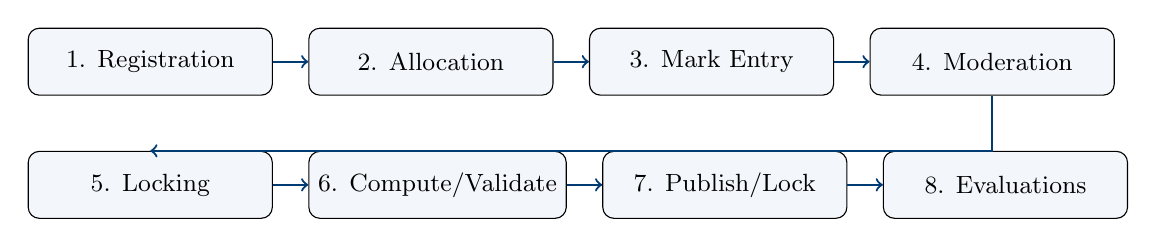
\begin{tikzpicture}[node distance=0.75cm, every node/.style={font=\small}]
  \node[draw, rounded corners, fill=irmsLight, minimum width=3.1cm, minimum height=0.85cm] (r1) {1. Registration};
  \node[draw, rounded corners, fill=irmsLight, right=0.45cm of r1, minimum width=3.1cm, minimum height=0.85cm] (r2) {2. Allocation};
  \node[draw, rounded corners, fill=irmsLight, right=0.45cm of r2, minimum width=3.1cm, minimum height=0.85cm] (r3) {3. Mark Entry};
  \node[draw, rounded corners, fill=irmsLight, right=0.45cm of r3, minimum width=3.1cm, minimum height=0.85cm] (r4) {4. Moderation};

  \node[draw, rounded corners, fill=irmsLight, below=0.7cm of r1, minimum width=3.1cm, minimum height=0.85cm] (r5) {5. Locking};
  \node[draw, rounded corners, fill=irmsLight, right=0.45cm of r5, minimum width=3.1cm, minimum height=0.85cm] (r6) {6. Compute/Validate};
  \node[draw, rounded corners, fill=irmsLight, right=0.45cm of r6, minimum width=3.1cm, minimum height=0.85cm] (r7) {7. Publish/Lock};
  \node[draw, rounded corners, fill=irmsLight, right=0.45cm of r7, minimum width=3.1cm, minimum height=0.85cm] (r8) {8. Evaluations};

  \draw[->, thick, color=irmsBlue] (r1) -- (r2);
  \draw[->, thick, color=irmsBlue] (r2) -- (r3);
  \draw[->, thick, color=irmsBlue] (r3) -- (r4);
  \draw[->, thick, color=irmsBlue] (r4.south) |- (r5.north);
  \draw[->, thick, color=irmsBlue] (r5) -- (r6);
  \draw[->, thick, color=irmsBlue] (r6) -- (r7);
  \draw[->, thick, color=irmsBlue] (r7) -- (r8);
\end{tikzpicture}
\end{center}
\vspace{0.25cm}
\centering
\textbf{Principle: Every stage has explicit controls before moving to the next stage.}
\end{frame}

\begin{frame}{Technology and Platform Architecture}
\begin{columns}[T]
\column{0.52\textwidth}
\textbf{Technology Baseline}
\begin{itemize}
  \item Laravel 12.48.1, PHP 8.3
  \item Blade + Alpine.js front-end
  \item Tailwind CSS 4, Vite build pipeline
  \item SQLite operational database
  \item Filament v3 for admin resources
\end{itemize}

\column{0.48\textwidth}
\textbf{Architecture Style}
\begin{itemize}
  \item CRUD modules for master/reference data
  \item Workflow modules for lifecycle-heavy operations
  \item Policy + gate enforcement for sensitive actions
  \item Audit-log oriented governance model
\end{itemize}
\end{columns}

\vspace{0.25cm}
\begin{block}{Design Outcome}
Balance between operational speed (workflow pages) and maintainability (admin resources and policy-driven control).
\end{block}
\end{frame}

\begin{frame}{Core Functional Modules (What Zones Use)}
\small
\begin{tabularx}{\textwidth}{>{\RaggedRight\arraybackslash}p{3.0cm} X}
\toprule
\textbf{Module} & \textbf{Scope and Value} \\
\midrule
Registration & Candidate, school, district, and exam-year enrollment with scope control. \\
ACSEE Allocation & Combination/subject allocation and private-candidate subject assignment workflows. \\
Mark Entry & CSV/ZIP ingestion, validation, batch lifecycle, moderation, approval, lock/unlock. \\
Results Processing & Compute/validate, grading profile control, publish/lock snapshots, admin unlock. \\
Evaluations & School/council/district/region views, rankings, outlier/extremity analytics. \\
Governance \& Backup & Authentication auditing, action trails, backup/restore with restore audit logs. \\
\bottomrule
\end{tabularx}
\end{frame}

\begin{frame}{ACSEE Mark Entry Workflow (Operational View)}
\begin{enumerate}
  \item Select context (exam year, region, district, school, subject).
  \item Download template (paper structure and format constraints).
  \item Upload marks (CSV/ZIP) into draft batch.
  \item Run validation (candidate link, subject registration, paper completeness, ranges).
  \item Send for moderation; resolve flagged errors/incidents.
  \item Approve and lock batch (immutable stage for compute readiness).
\end{enumerate}

\vspace{0.25cm}
\begin{block}{Control Principle}
No progression to compute stage without passing lifecycle gates and data-quality checks.
\end{block}
\end{frame}

\begin{frame}{Data Quality and Compute Rules}
\begin{itemize}
  \item Subject marks normalized to 100 using configured paper weights.
  \item Compute policy rounds normalized subject marks to whole numbers.
  \item Canonical paper maxima: Paper 1/2 = 100, Paper 3 = 50 (unless configured).
  \item Irregular statuses handled explicitly: INC, ABS, X with priority logic.
  \item Readiness indicators depend on promoted/valid marks, not only uploaded rows.
\end{itemize}

\vspace{0.2cm}
\begin{alertblock}{Operational Benefit}
Stronger consistency across schools and councils; fewer disputes during publication and post-publication review.
\end{alertblock}
\end{frame}

\begin{frame}{Security, Authorization, and Accountability}
\begin{columns}[T]
\column{0.5\textwidth}
\textbf{Access Control}
\begin{itemize}
  \item Custom RBAC with role + scope binding
  \item Region/district/school isolation
  \item Policy and gate checks for critical actions
  \item Password-change enforcement and status control
\end{itemize}

\column{0.5\textwidth}
\textbf{Governance Controls}
\begin{itemize}
  \item Authentication and action audit logging
  \item Moderation and unlock actions are recorded
  \item Publish/lock and admin-unlock events traceable
  \item Backup and restore actions audited
\end{itemize}
\end{columns}
\end{frame}

\begin{frame}{Results Governance: Publish, Lock, Unlock}
\begin{itemize}
  \item Compute runs generate versioned results artifacts.
  \item Publication is separated from locking to support governance review.
  \item Locking protects final output from accidental mutation.
  \item Admin unlock exists for controlled exception handling (with reason trail).
  \item Snapshot/version workflow supports defensible result history.
\end{itemize}
\vspace{0.2cm}
\begin{block}{Leadership Value}
Decisions are reversible only through governed pathways, not ad-hoc edits.
\end{block}
\end{frame}

\begin{frame}{Live Operational Snapshot (Database, Feb 27, 2026)}
\small
\begin{tabularx}{\textwidth}{>{\RaggedRight\arraybackslash}p{6.0cm} >{\RaggedLeft\arraybackslash}X}
\toprule
\textbf{Indicator} & \textbf{Current Count} \\
\midrule
Regions in scope & 8 \\
Districts in scope & 19 \\
Registered schools & 93 \\
Candidate master records & 11,168 \\
ACSEE registrations (2026) & 11,168 \\
ACSEE subject selections (2026) & 48,299 \\
ACSEE mark-import batches (2026 total) & 581 \\
Locked ACSEE batches (2026) & 551 \\
Active result runs (pending/in\_progress) & 0 \\
Latest result run (ID 30) & completed, 8,973/8,973 processed \\
\bottomrule
\end{tabularx}
\vspace{0.2cm}
\footnotesize Source: local production-aligned database snapshot generated at 2026-02-27 03:26.
\end{frame}

\begin{frame}{System Strengths for Zonal Operations}
\begin{enumerate}
  \item \textbf{Traceability}: full lifecycle visibility from upload to publication.
  \item \textbf{Control}: moderation, lock, unlock, and publication governance.
  \item \textbf{Data quality}: strict validation and irregularity handling.
  \item \textbf{Scalability of operations}: bulk import and scope-based filtering.
  \item \textbf{Transparency}: public and internal result views with aligned logic.
  \item \textbf{Audit readiness}: defensible logs for compliance and incident response.
\end{enumerate}
\end{frame}

\begin{frame}{Key Risks and Improvement Priorities}
\begin{itemize}
  \item \textbf{Role-system consistency}: continue hardening one authorization model across all controllers.
  \item \textbf{Operational resilience}: strengthen stale-run auto-recovery and queue/worker observability.
  \item \textbf{Database growth path}: plan migration path for higher write concurrency when scale rises.
  \item \textbf{UI clarity}: continue reducing ambiguity in lifecycle labels and readiness counters.
  \item \textbf{Institutional readiness}: keep zonal training and SOP updates synchronized with releases.
\end{itemize}
\vspace{0.15cm}
{\footnotesize Evidence source includes architecture and lifecycle audit documentation in repository.}
\end{frame}

\begin{frame}{90-Day Action Plan (Zonal Focus)}
\small
\begin{tabularx}{\textwidth}{>{\RaggedRight\arraybackslash}p{1.4cm} >{\RaggedRight\arraybackslash}p{3.7cm} X}
\toprule
\textbf{Window} & \textbf{Priority} & \textbf{Expected Outcome} \\
\midrule
0--30 days & Lifecycle reliability hardening & Fewer stuck runs, faster operator recovery, clearer readiness status. \\
31--60 days & Authorization consistency pass & Reduced permission edge cases and stronger governance confidence. \\
61--90 days & Scale and reporting optimization & Better performance under peak loads and improved zonal monitoring dashboards. \\
\bottomrule
\end{tabularx}
\vspace{0.25cm}
\begin{block}{Execution Model}
Joint workstream: Zonal operations + system team + governance focal persons.
\end{block}
\end{frame}

\begin{frame}{What We Need From Zonal Leadership}
\begin{itemize}
  \item Confirm standard operating procedures for exception handling (unlock/recompute/escalation).
  \item Nominate zonal super-users for rapid support and training-of-trainers.
  \item Approve periodic operational review cadence (weekly in exam season).
  \item Endorse phased hardening priorities and milestone tracking.
\end{itemize}

\vspace{0.4cm}
\centering
\Large\textbf{IRMS is ready for controlled scale-up with governance-first execution.}
\end{frame}

\begin{frame}{Appendix: Source Artifacts Used}
\footnotesize
\begin{itemize}
  \item \texttt{docs/IRMS\_ADMIN\_PANEL\_ARCHITECTURE\_REPORT.md}
  \item \texttt{MARK\_ENTRY\_WORKFLOWS.md}
  \item \texttt{COMPLETE\_SYSTEM\_SUMMARY.md}
  \item \texttt{app/Http/Controllers/Api/Results/AcseeLifecycleApiController.php}
  \item Live DB snapshot queries executed via \texttt{php artisan tinker} on 2026-02-27.
\end{itemize}
\vspace{0.25cm}
\textbf{Note}: Update the snapshot slide before final delivery if new data is loaded.
\end{frame}

\begin{frame}
\centering
\Huge Thank You
\vspace{0.4cm}

\Large Questions \& Discussion
\end{frame}

\end{document}
